% !TEX Root = ../proposal.tex

\section*{Research Challenges}
\subsection*{Previous approaches}

\begin{frame}{Challenges for Optimal Transfer Design} %-----------------------------%

\begin{itemize}
    \item Optimal Trajectory Design
        \begin{itemize}
            \item Orbital dynamics are nonlinear and chaotic
            \item Very sensitive to initial conditions
            \item Intuition required by designer to enable convergence
        \end{itemize}
    \pause
    \item Transfers using low-thrust propulsion
        \begin{itemize}
            \item Requires long periods of thrusting/coasting
            \item Small perturbations require accurate numerical integration
            \item Difficult to capture the long-term effects accurately
        \end{itemize}
    \pause
    \item Direct Optimal Control
        \begin{itemize}
            \item Reformulate problem as parameter optimization
            \item Allows for use of nonlinear programming methods
            \item High dimensional problem and computationally intensive
            \item Results in suboptimal solutions due to discretization
        \end{itemize}
\end{itemize}
\end{frame}   %-----------------------------%

\begin{frame}
\frametitle{Gravitational Modeling}
\begin{block}{Centrobaric Body}
    \( F = -\frac{G m_1 m_2}{R^2} \hat{a}_1 \) for all particles outside of body
\end{block}

\begin{itemize}
    \item<2-> Only applies to spherically symmetric bodies 
    \item<3-> Unknown or possibly changing mass distributions
    \item<4-> Can derive a \Emph{Gravity Model} using accurate tracking of SC
\end{itemize}
\only<4>{
\[
    U = \frac{\mu}{r} \sum_{n=0}^\infty \sum_{m=0}^\infty \parenth{\frac{R}{r}}^nP_{n,m}(\sin \phi) \braces{ C_{nm} \cos(m \lambda) + S_{nm} \sin(m \lambda)} 
\]
}
\note[itemize]{
    \item Models require detailed data from orbit about asteroid (OD process determines gravity field)
    \item Simplified models (triaxial ellipsoid allows analytical insight)
    \item Previous work fails to consider coupled dyanmics
    }
\end{frame}

\begin{frame}
\frametitle{Dynamic System Modelling}
\begin{itemize}
    \item Astrodynamics - motion of particles due to gravity
    \item Attitude coupling is dependent on ratio \( \epsilon = \frac{l}{R} \)
        \begin{itemize}
            \item Typically ignored for Earth based missions 
            \item Force depends on attitude and oment depends on position
            \item Vastly different time scales
        \end{itemize}
\end{itemize}
\begin{align*}
    m \dot{v} &= m v \times \Omega + \sum F(b, R) \\
    J \dot{\Omega}  &= J \Omega \times \Omega +  \sum M(b, R) 
\end{align*}

\begin{center}
    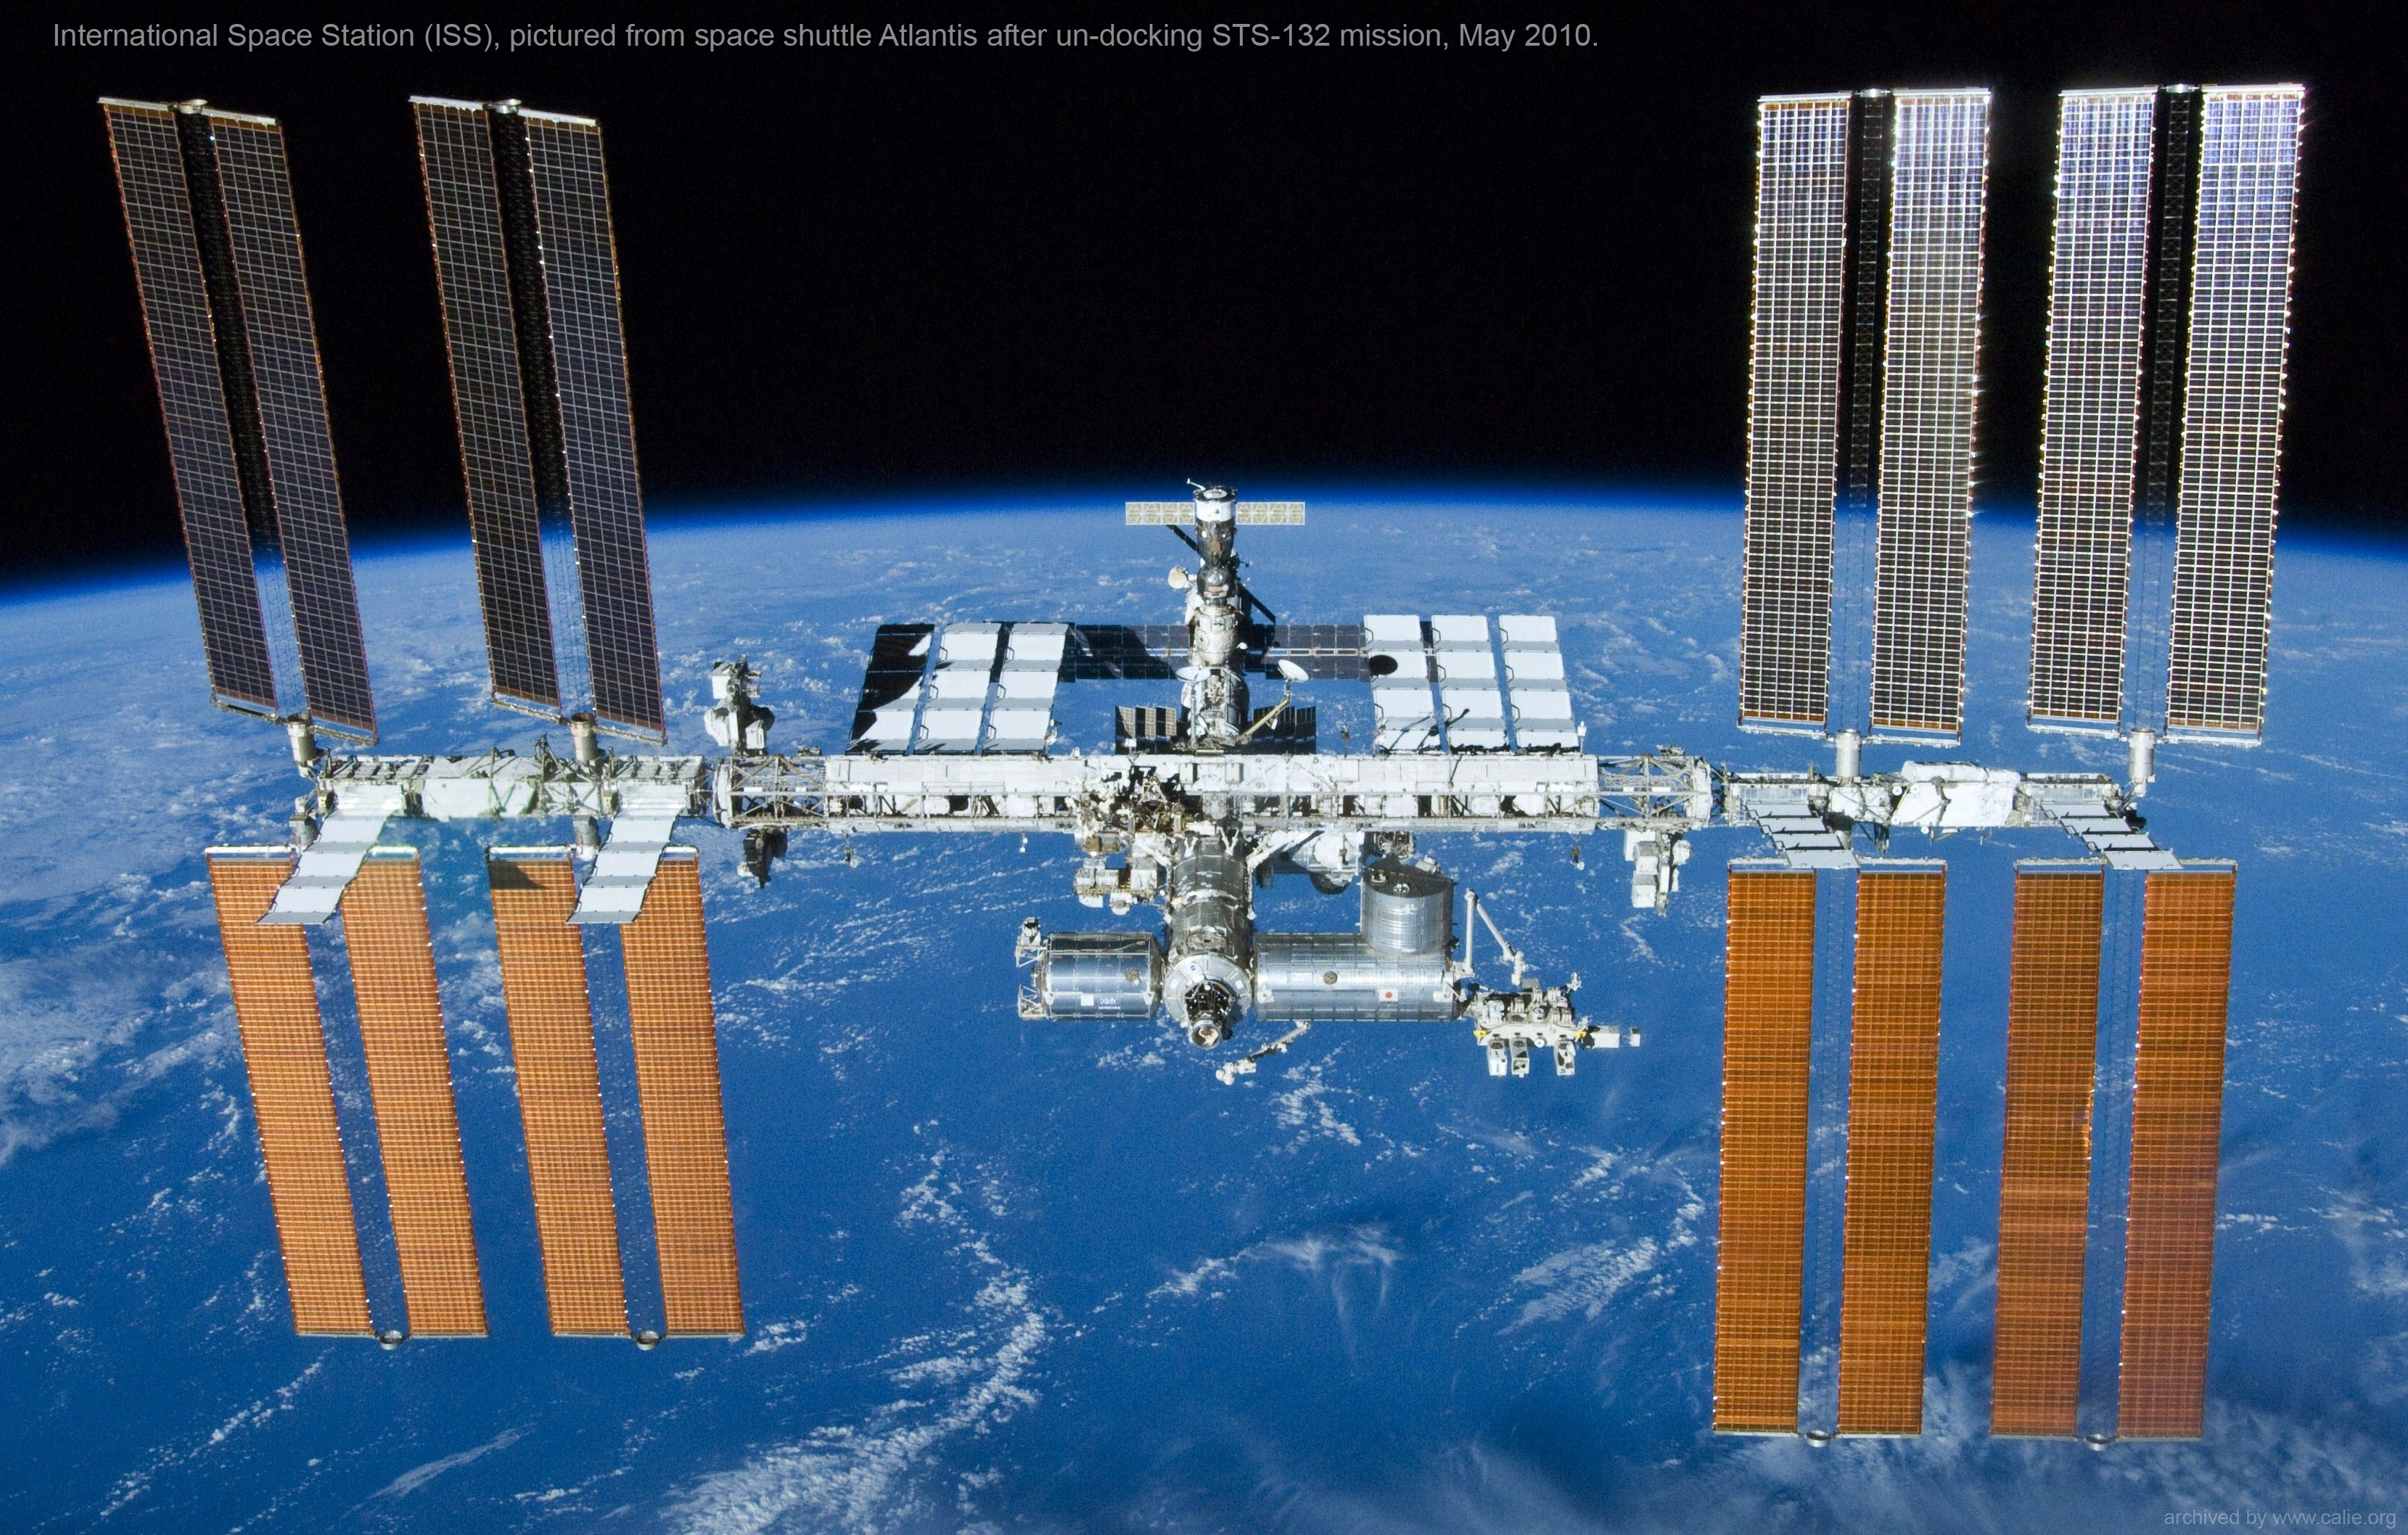
\includegraphics[width=0.5\textwidth,height=0.4\textheight,keepaspectratio]{figures/ISS_STS-132.jpg}
    \quad
    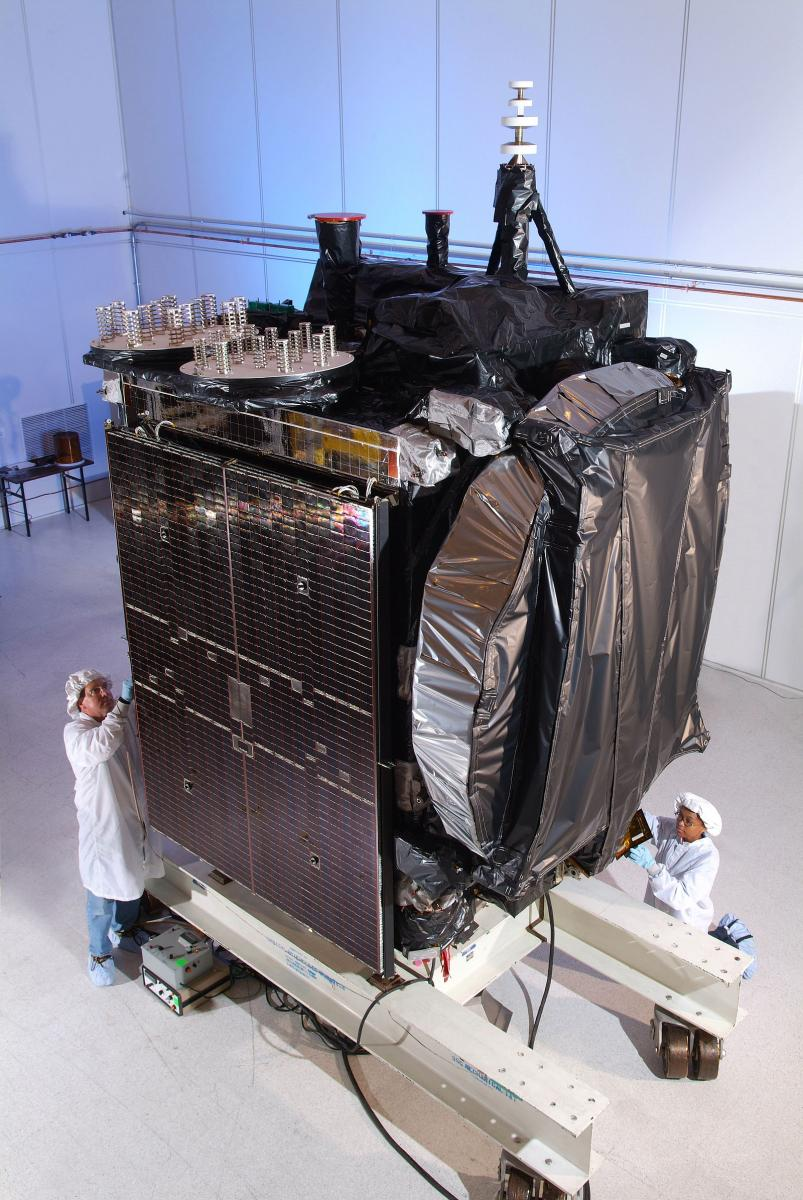
\includegraphics[width=0.5\textwidth,height=0.4\textheight,keepaspectratio]{figures/Galaxy_15_photo.jpg}
\end{center}

\note[itemize]{
    \item Galaxy-15 is about a \SI{2}{\meter} cube, \SI{2500}{\kilo\gram}
    \item Located in GEO at \SI{133}{\degree} W
}
\end{frame}


\begin{frame}[t]{Planetary Landing} %-----------------------------------%
\begin{center}
    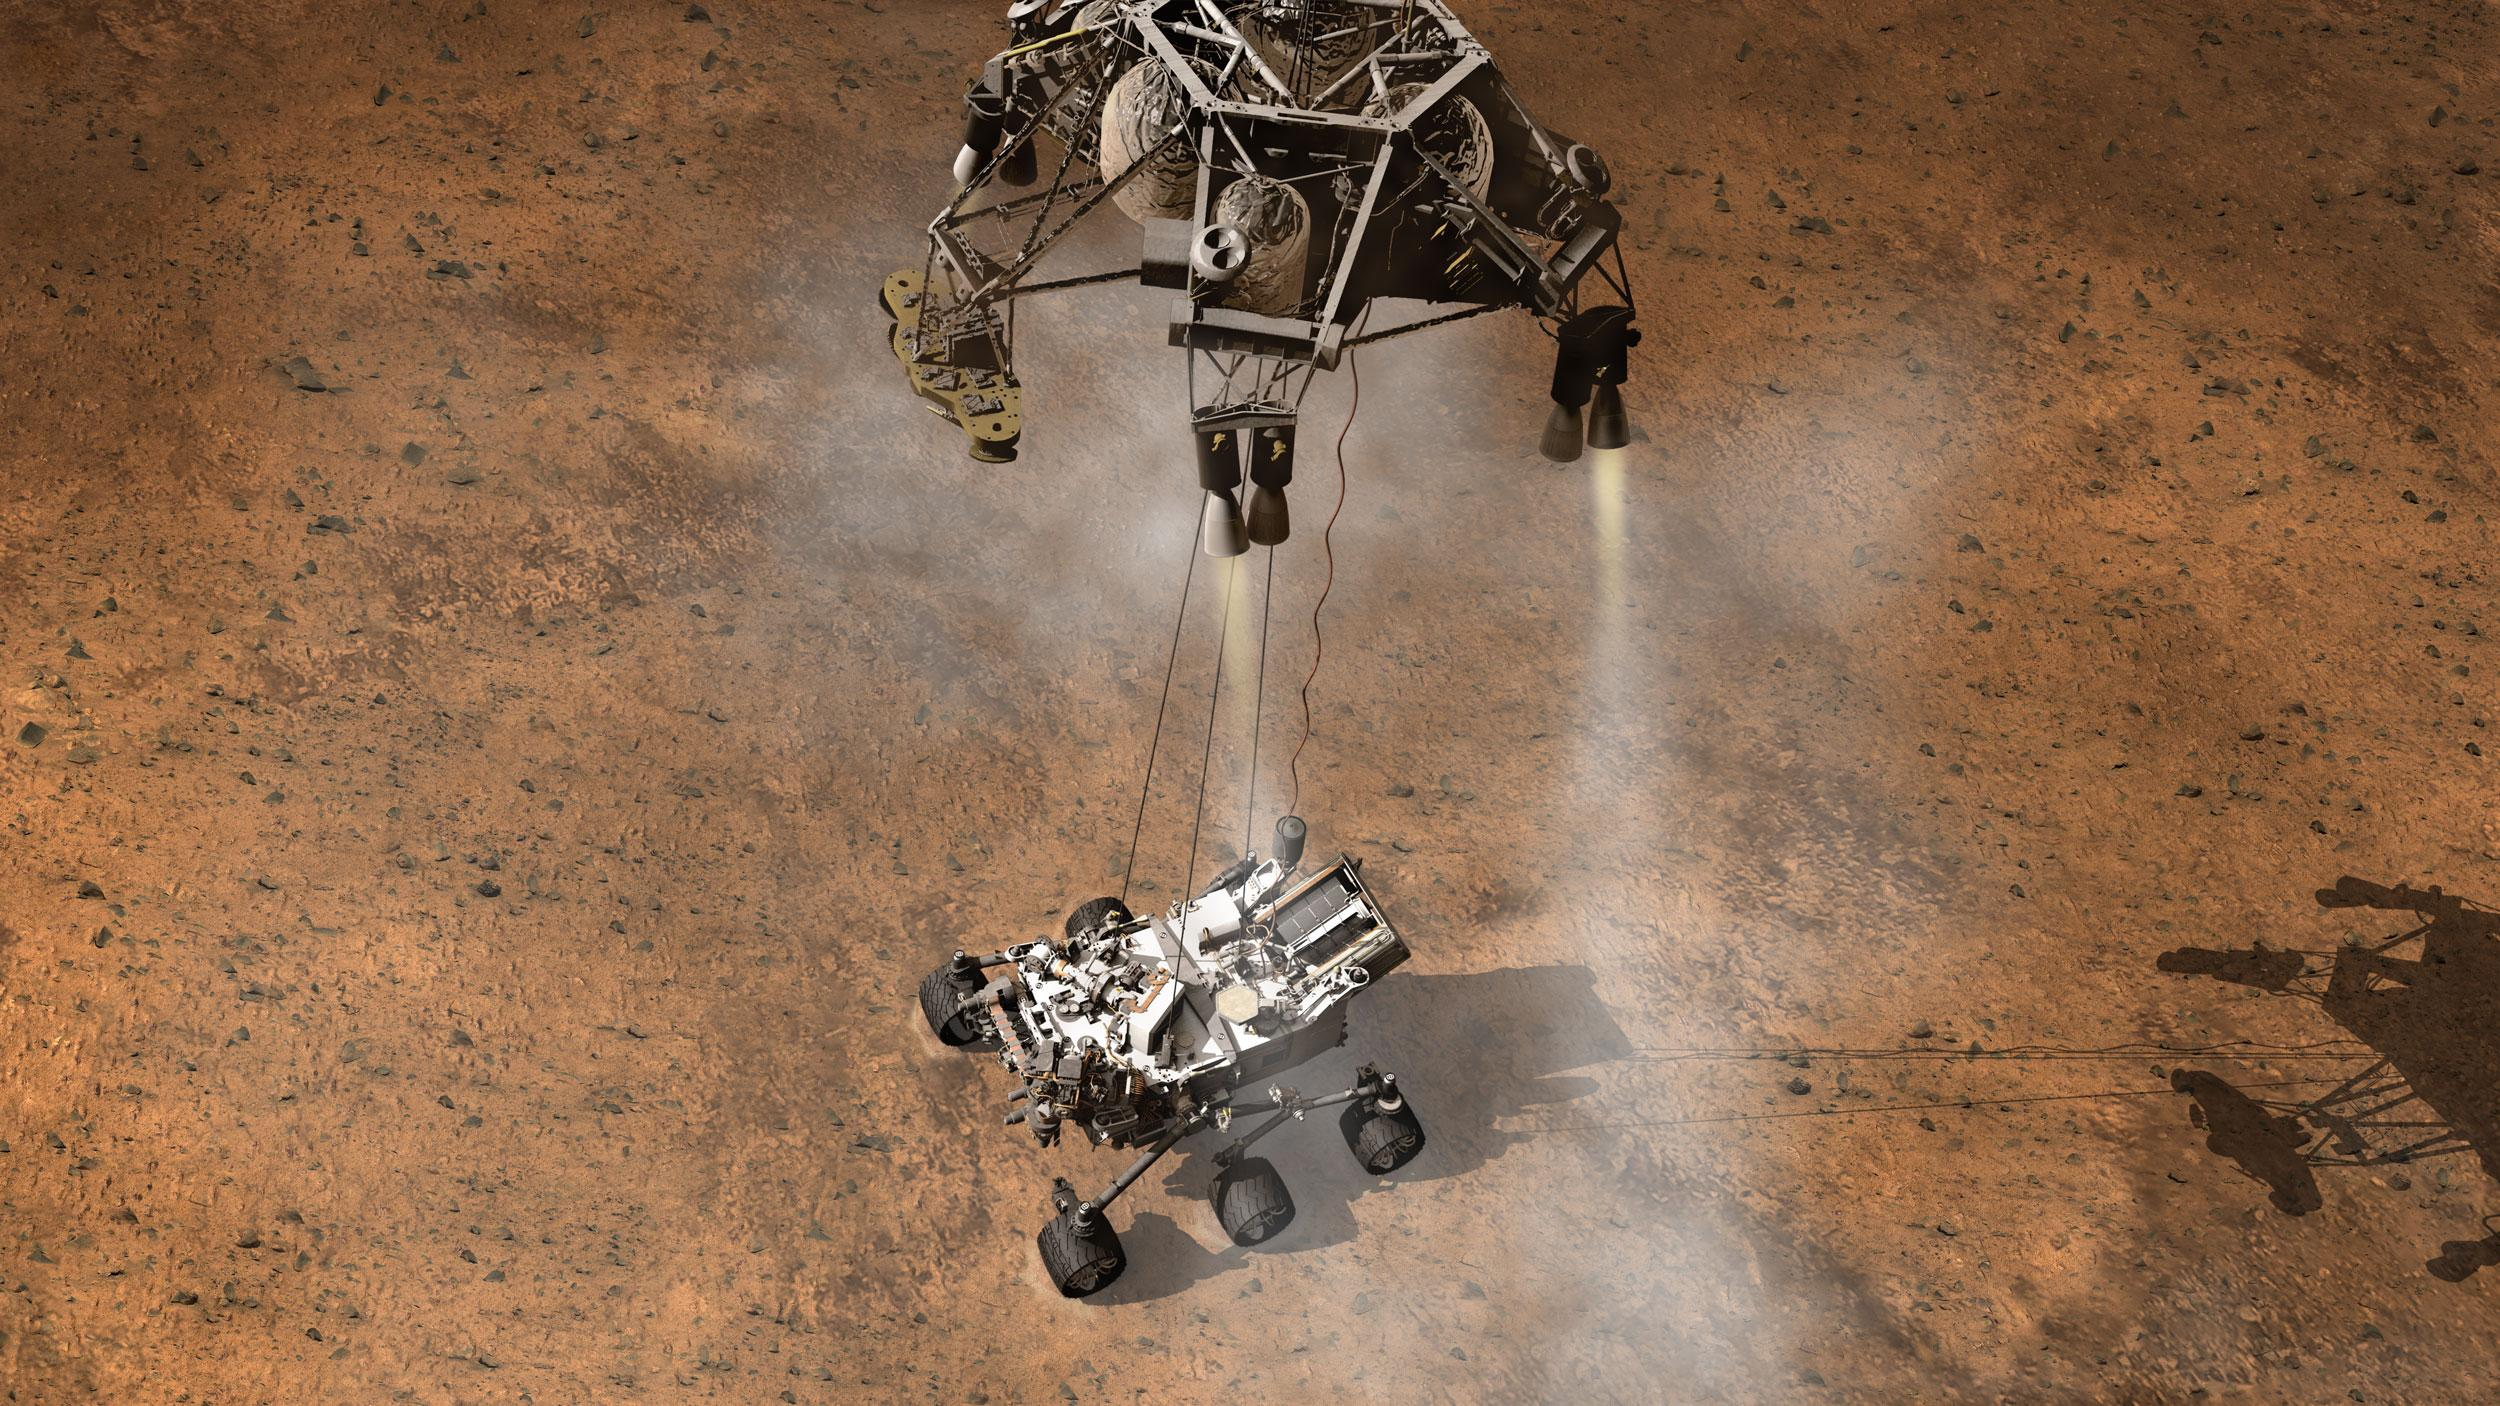
\includegraphics[width=0.5\textwidth,height=0.3\textheight,keepaspectratio]{figures/curiosity.jpg} ~
    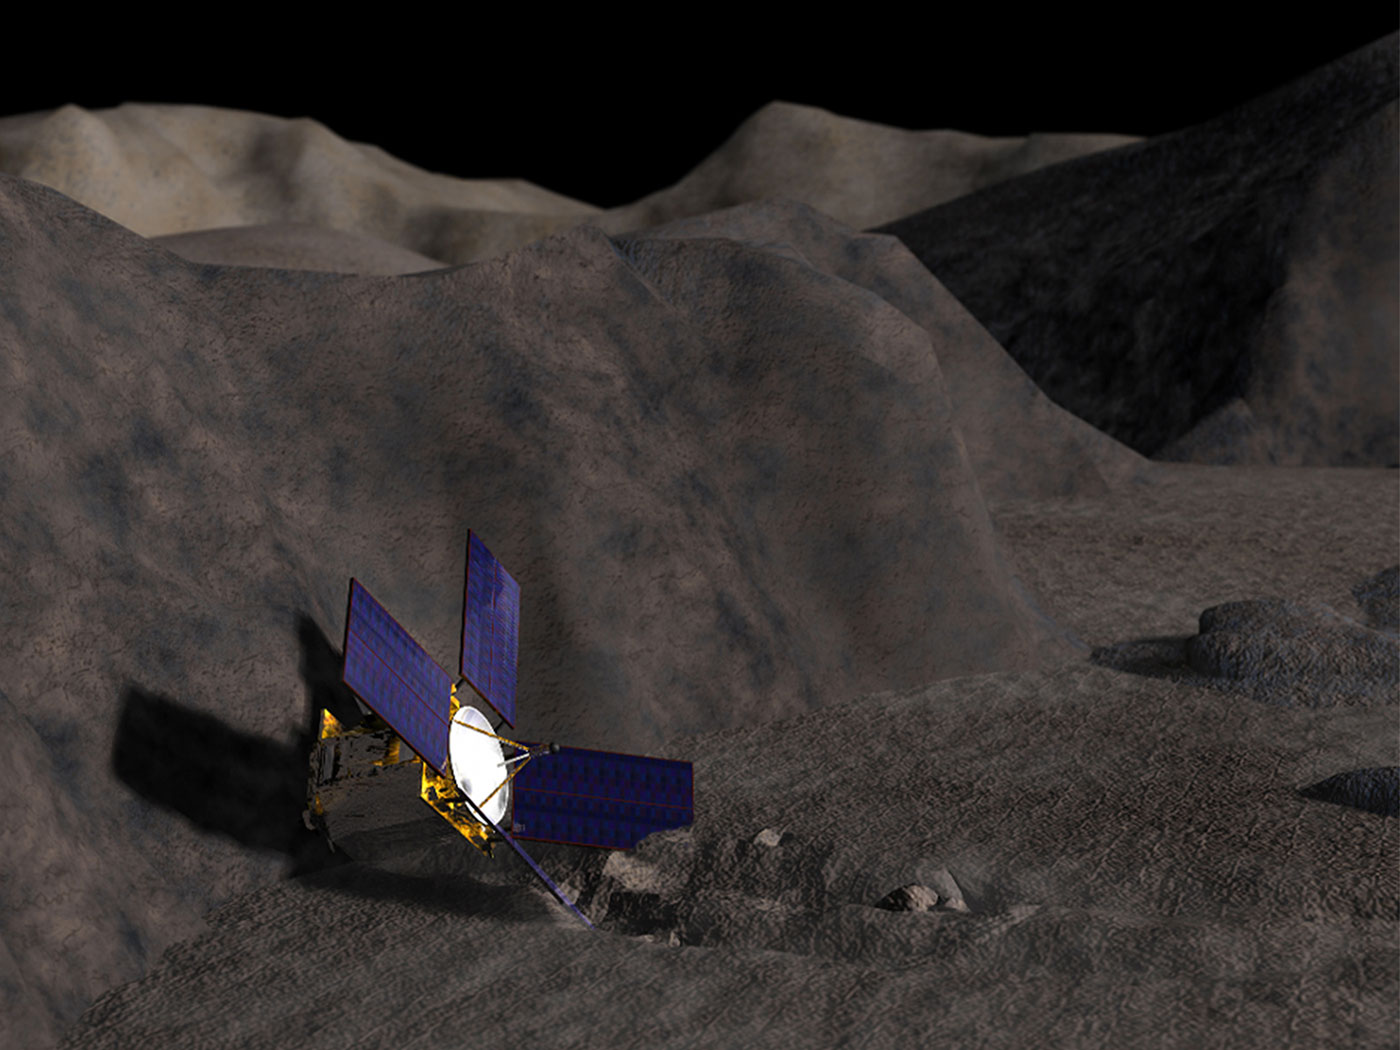
\includegraphics[width=0.5\textwidth,height=0.3\textheight,keepaspectratio]{figures/430_new_landingnearstill.jpg}
\end{center}

\begin{itemize}
    \item Extensive history of manned/unmanned planetary landings
    \item Previous approaches highly resource dependent
    \begin{itemize}
        \item Optimization based appraoch
        \item Extensive human planning
    \end{itemize}
    \item All methods not robust to obstacles/failures
\end{itemize}

\begin{frame}{Attitude Parameterizations}
    \begin{itemize}
        \item Euler Angles
        \begin{itemize}
            \item Minimal representation used for small attitude changes.
            \item Singularities exist for large angle slews: requires switching between 24 sequences
            \item Complicated trigonometric functions
        \end{itemize}
        \pause
        \vs
        \item Quaternion 
        \begin{itemize}
            \item No singularities
            \item Two anti-podal quaternions for the same attitude
            \item Unwinding behavior for control systems
        \end{itemize}
        \pause
        \vs
        \item Geometric control
        \begin{itemize}
            \item Globally and uniquely characterize attitude: \( R \in \SO \)
            \item Controller is globally valid for large angle maneuvers
        \end{itemize}
    \end{itemize}
    
\end{frame}